\documentclass[12pt, letterpaper]{article}
\usepackage[utf8]{inputenc}
\usepackage{graphicx}
\usepackage{floatrow}

\usepackage[margin=2cm]{geometry} 



\renewcommand*\contentsname{Indholdsfortegnelse}

\begin{document}

\begin{titlepage}

\newcommand{\HRule}{\rule{\linewidth}{0.5mm}} % Defines a new command for the horizontal lines, change thickness here

\center % Center everything on the page
 
%----------------------------------------------------------------------------------------
%	HEADING SECTIONS
%----------------------------------------------------------------------------------------

\textsc{\LARGE Aarhus universitet}\\[1.5cm] % Name of your university/college
\textsc{\Large DSB}\\[0.5cm] % Major heading such as course name
\textsc{\large Semester 3}\\[0.5cm] % Minor heading such as course title

%----------------------------------------------------------------------------------------
%	TITLE SECTION
%----------------------------------------------------------------------------------------

\HRule \\[0.4cm]
{ \huge \bfseries Mini-projekt - Del 3}\\[0.4cm] % Title of your document
\HRule \\[1.5cm]
 
%----------------------------------------------------------------------------------------
%	AUTHOR SECTION
%----------------------------------------------------------------------------------------

% If you don't want a supervisor, uncomment the two lines below and remove the section above
\Large \emph{Studerende:}\\[1cm]
Mette \textsc{Hammer Nielsen-Kudsk - Studienr: 201408391}\\[0,5cm] % Your name
Martin \textsc{Banasik - Studienr: 201408398}\\[0,5cm] % Your name
Finja \textsc{Jette Ralfs - Studienr: 201303659}\\[0,5cm] % Your name
%----------------------------------------------------------------------------------------
%	DATE SECTION
%----------------------------------------------------------------------------------------

{\large Oktober 5, 2015}\\[1,2cm] % Date, change the \today to a set date if you want to be precise

%----------------------------------------------------------------------------------------
%	LOGO SECTION
%----------------------------------------------------------------------------------------


\includegraphics[scale=0.5]{billeder/au}\\ % Include a department/university logo - this will require the graphicx package
 
 %\includegraphics[width=0.6\textwidth]{figurer/ASE}~\\[1cm]
%----------------------------------------------------------------------------------------

\vfill % Fill the rest of the page with whitespace


\end{titlepage}

\tableofcontents
\newpage

\newpage

\section{FIR - Finite impulse response}

En vægtet sum (udglatning, midling), som kører hen over input-signalet x(n). 

Differensligning for filteret og definition: 
$$ y(n)= \sum\limits_{k=0}^{M-1} b_k * x(n-k)$$

hvor, 
$$ x(n) = input $$
$$ y(n) = output $$
$$ b_k = filterets koefficienter $$ 
$$ M = filterets længde $$
$$ M-1 = filterets orden $$

\begin{figure}[!h]
           \begin{floatrow}
             \ffigbox{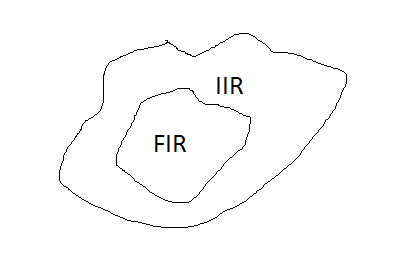
\includegraphics[width=1.1\linewidth]{billeder/domane}}		   			{\caption{FIR filter hører under IIR.}}
           \end{floatrow}
\end{figure}


\section{IIR - Infinite impulse response}

\section{Foldning}
Hvis vi ønsker at koble flere filter sammen, benytter vi kobling. 

Definition: 

$$ y(n)= \sum\limits_{k=0}^{M-1} h_k * x(n-k) $$

I MatLab benytter vi, ved foldning, funktionen "conv". 
Hvis vi har to signaler vi vil have koblet sammen, så repræsenteres dette ved en stjerne: 

\begin{center}
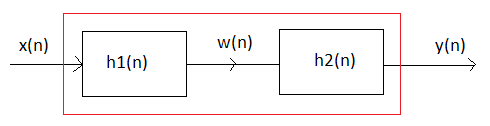
\includegraphics[width=0.7\textwidth]{billeder/foldning}
\end{center}

Den røde firkant omkredser de to signaler, der bliver foldet sammen. 

$$ h_1(n)\star h_2(n) $$


\section{Impulsfunktion: $\delta(n)$}

\section{Impulsrespons og overføringskarakteristik}


\section{Vindues metoden}
Når vi analytisk skal designe et filter, benytter vi os af vinduesmetoden. Her befinder vi os i frekvensverden (DFT). 
1) Vi specificer det ønskede frekvens karakteristik.
2) Herefter laver vi Invers DFT (IDFT). 
3) Så ganger vi vinduet på. 
4) Til sidst tjekker vi frekvenskarakteristik med DFT. 
 
\section{Filter design i MatLab}
Vi benytter os af to forskellige funktioner "fir1" og "fir2". 

- "fir1": 
$$ b = fir1(N, \frac{f_C}{0,5*f_s}, 'high') $$ 
hvor, 
$$ f_C = knækfrekvensen $$
$$ f_s = samplesfrekvens $$

Her vil MatLab lave et højpas filter, da vi har indskrevet 'high'. 
Hvis vi ønskede et lavpas filter skulle vi ikke havde skrevet noget. Ønskede vi et båndpas filter, ville vi skulle skrive bandpas og ved båndstop filer, bandstop. 

- "fir2": 
$$ b = fir2(N, ..., ...) $$
Her skal der indsættes amplituder. Benyt "help" funktionen i MatLab foran "fir2", hvis der ønskes mere information om denne funktion. 

\section{Fremtidigt arbejde}
 
\section{Konklusion}


\end{document}